\baitraloingan{De01TLN:01}{
	Cho hàm số $f(x)=x-3+\frac{1}{x-2}$. Tìm giá trị nhỏ nhất của hàm số đã cho trên $(2;+\infty)$.
}{
	\dapantln{1}{}{}{}
}{
	{\bfseries Lời giải:}
	
	Xét hàm số $f(x)=x-3+\frac{1}{x-2}$ trên $(2;+\infty)$.
	
	$f'(x)=1-\frac{1}{(x-2)^{2}}=0\Rightarrow x=3\in (2;+\infty)$. Ta có bảng biến thiên của hàm số trên $(2;+\infty)$ như sau:
	
	\centerline{
		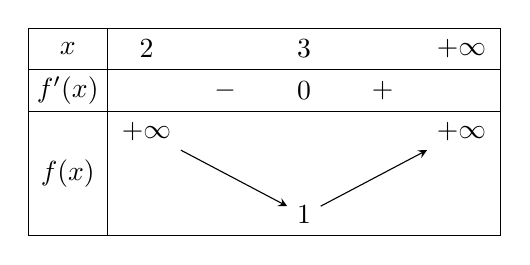
\begin{tikzpicture}[y=1.5em]
			\foreach \x/\gt in {0/x,1/2,3/3,5/+\infty}\path (\x,0) node{$\gt$};
			\foreach \x/\gt in {0/f'(x), 2/-,3/0,4/+}\path (\x,-1) node{$\gt$};
			\foreach \x/\y/\gt[count=\i from 0] in {0/-3/f(x),1/-2/+\infty,3/-4/1,5/-2/+\infty}\path (\x,\y) node(\i){$\gt$};
			\foreach \x/\y in {1/2,2/3}\draw[-stealth] (\x)--(\y);
			\draw (-.5,.5) rectangle (5.5,-4.5) (-.5,-.5)--(5.5,-.5) (-.5,-1.5)--(5.5,-1.5) (.5,.5)--(.5,-4.5);
		\end{tikzpicture}
	}
	
	Từ bảng biến thiên suy ra giá trị nhỏ nhất của hàm số $f(x)$ là $f(3)=1$.
}

\baitraloingan{De01TLN:02}{
	Cho hàm số $f(x)=x^{3}+3x^{2}-1$. Đồ thị hàm số có các điểm cạc đại, cực tiểu lần lượt là $A$ và $B$. Tính độ dài đoạn thẳng $AB$.
}{
	\dapantln{4}{,}{4}{7}
}{
	Hàm số $f(x)$ có đạo hàm $f'(x)=3x^{2}+6x$. $f'(x)$ có hai nghiệm $x=0$ và $x=-2$. Tương ứng các điểm $A(0;-1)$ và $B(-2;3)$.
	
	Do đó $AB=\sqrt{(-2-0)^{2}+(3-(-1))^{2}}=\sqrt{20}\simeq 4,47$.
}

\baitraloingan{De01TLN:03}{
	Một bác nông dân có mảnh vườn hình chữ nhật với chiều sâu $50$ mét, chiều rộng $20$ mét và $60$ mét lưới. Bác dự định căng lưới làm hàng rào để nuôi gà, lợi dụng một mặt tường bao dài $50$ mét nên bác chỉ cần căng lưới ba chiều còn lại. Tính diện tích lớn nhất mà bác nông dân có thể nuôi gà (tham khảo hình vẽ dưới đây)
	
	\centerline{
		\begin{tikzpicture}
			\draw[dashed] (0,5)--(0,0) node[pos=.5,left]{$50$ (m)}--(2,0) node[pos=.5,below]{$20$ (m)}--(2,5)--cycle; 
			\draw (0,5)--(1.5,5)--(1.5,3.5)--(0,3.5);
			\draw[-stealth] (1.5,4)--++(0:2) node[right]{lưới};
		\end{tikzpicture}
	}
}{
	\dapantln{2}{0}{0}{}
}{
	
}

\baitraloingan{De01TLN:04}{
	Sau khi đăng quang cuộc thi hoa hậu hoàn vũ Việt Nam năm 2024, một nhóm người
	đẹp đi làm từ thiện gồm có Hoa hậu, Á hậu 1 và Á hậu 2. Biết rằng nhóm sẽ không đi làm từ
	thiện nếu Hoa hậu rời nhóm hoặc cả hai Á hậu cùng rời nhóm. Khả năng để Hoa hậu, Á hậu
	1, Á hậu 2 rời nhóm lần lượt là $\frac{1}{4}$; $\frac{1}{5}$ và $\frac{3}{10}$. Biết các quyết định rời nhóm của Hoa hậu và các Á hậu độc lập nhau. Xác suất để nhóm có thể đi làm từ thiện bằng bao nhiêu?
}{
	\dapantln{0}{,}{7}{1}
}{
	{\bfseries Lời giải}
	
	Gọi $A$ là biến cố: Nhóm có thể đi làm từ thiện.
	
	$A_{1}$ là biến cố : Hoa hậu rời nhóm; $A_{2}$ là biến cố: Á hậu 1 rời nhóm; $A_{3}$ là biến cố: Á hậu 2 rời nhóm.
	
	Ta có: $A=\overline{A_{1}A_{2}A_{3}}\cup \overline{A_{1}}A_{2}\overline{A_{3}}\cup \overline{A_{1}}\overline{A_{2}}A_{3}$.
	
	Khi đó $P(A)=\frac{3}{4}\cdot \frac{4}{5}\cdot\frac{7}{10}+\frac{3}{4}\cdot\frac{1}{5}\cdot\frac{7}{10}+\frac{3}{4}\cdot\frac{4}{5}\cdot\frac{3}{10}\simeq 0,71$.
}

\baitraloingan{De01TLN:05}{
	Trong không gian $Oxyz$ cho ba điểm $A(2;-1;1)$, $B(-1;3;-1)$ và $C(5;-3;3)$. Độ dài đường trung tuyến $AM$ của tam giác $ABC$ bằng bao nhiêu?
}{
	\dapantln{4}{,}{4}{7}
}{
	{\bfseries Lời giải:}
	
	$M$ là trung điểm của $BC$ nên $M(2;3;1)$.
	
	Suy ra $AM=\sqrt{(2-2)^{2}+(3-(-1))^{2}+(3-1)^{2}}=\sqrt{20}\simeq 4,47$
}

\baitraloingan{De01TLN:06}{
	Thống kê số thẻ vàng của các câu lạc bộ bóng đá trong giải V-league 2023 (gồm 14 đội bóng) có kết quả như sau:
	
	\centerline{
		\begin{tabular}{|c|c|c|c|c|c|c|}
			\hline
			$49$ & $79$ & $59$ & $52$ & $68$ & $73$ & $45$ \\
			\hline
			$39$ & $61$ & $60$ & $59$ &$52$ & $41$ & $40$ \\
			\hline
		\end{tabular}
	}
	
	Tìm khoảng biến thiên của mẫu số liệu ghép nhóm có độ dài bằng nhau với nhóm đầu tiên là $[30;40)$.
}{
	\dapantln{5}{0}{}{}
}{
	Ta có mẫu số liệu ghép nhóm như bảng sau:
	
	\centerline{
		\begin{tabular}{|c|c|c|c|c|c|}
			\hline
			Nhóm & $[30;40)$ & $[40;50)$ & $[50;60)$ & $[60;70)$ & $[70;80)$ \\
			\hline
			Tần số & $1$ & $4$ & $4$ & $3$ & $2$ \\
			\hline
		\end{tabular}
	}
	
	Khoảng biến thiên của mẫu số liệu ghép nhóm trên là $R=80-30=50$
}

\baitraloingan{De01TLN:07}{
	Trong không gian $Oxyz$, cho các điểm $A(0;3;-1)$ và $B(-1;-6;2)$. Gọi $C$ là giao điểm của đường thẳng đi qua $AB$ và trục $Ox$. Hoành độ của điểm $C$ bằng bao nhiêu? (kết quả được làm tròn đến hàng phần chục)
}{
	\dapantln{-}{0}{,}{3}
}{
	$C$ thuộc trục $Ox$ nên tọa độ của điểm $C$ có dạng $C(x;0;0)$. Khi đó ta có $\overrightarrow{AC}=(x;-3;1)$ và $\overrightarrow{AB}=(-1;-9;3)$.
	
	$C$ nằm trên đường thẳng qua $AB$ nên $\overrightarrow{AB}$ và $\overrightarrow{AC}$ cùng phương hay: $\frac{x}{-1}=\frac{-3}{-9}=frac{1}{3}\Rightarrow x=-\frac{1}{3}\simeq -0,3$.
}

\baitraloingan{De01TLN:08}{
	Dân số Việt Nam sau $t$ năm tính từ năm 2023 được dự đoán theo công thức $N(t)=100e^{0,012t}$ (triệu người), với $0<t\leq 50$. Biết rằng đạo hàm của hàm số $N(t)$ biểu thị tốc độ gia tăng dân số của Việt Nam (đơn vị là triệu người/năm). Sau ít nhất bao nhiêu năm (kể từ năm 2023) thì tốc độ gia tăng dân số của Việt Nam sẽ lớn hơn $2$ (triệu người/năm)? (kết quả tính tròn năm).
}{
	\dapantln{4}{3}{}{}
}{
	{\bfseries Lời giải:}
	
	Ta có: $N(t)=100e^{0,012t}\Rightarrow N'(t)=1,2e^{0,012t}$.
	
	Tốc độ gia tăng dân số lớn hơn $2$ (triệu người/năm) khi $N'(t)>2$.
	
	$\Leftrightarrow 1,2e^{0,12t}>2\Leftrightarrow t>42,56$.
	
	Như vậy, sau ít nhất $43$ năm thì tốc độ gia tăng dân số của Việt Nam sẽ lớn hơn $2$ (triệu người/năm).
}